%!TEX root = ../synopsis.tex

В {\bf третьей главе}
рассматривается задача непрерывной резки {\it CCP}
на Евклидовой плоскости
$\mathbb R \times \mathbb R$.
Возьмём
$N$
попарно непересекающихся плоских контуров
$\{C_1, C_2, ... C_N\}$,
ограничивающих
$n$
деталей
$\{A_1, A_2, ... A_n\}$.
В общем случае
$n \leqslant N$.
В данной работе рассматриваются только контуры
$C_i$,
состоящие из
(конечного числа)
отрезков прямых линий и дуг окружностей,
так как именно такие геометрические примитивы
поддерживаются программным обеспечением
современных машин термической резки с ЧПУ.
Выберем также две точки
$M_0$, $M_{N + 1}$
(почти всегда $M_0 = M_{N + 1}$),
которые будут использоваться
как начало и конец
маршрута резки.
Задача непрерывной резки
({\it Continuous Cutting Problem, CCP})
состоит в поиске:
\begin{enumerate}
\item
$N$ точек врезки $M_i \in C_i, i \in \overline{1, N}$
\item
Последовательности обхода контуров
$C_i$,
то есть перестановки
$N$
элементов
$I = (i_1, i_2, ... i_N)$
\end{enumerate}
Результатом решения задачи будет являться маршрут
\begin{equation}
  \label{eq:route}
  \mathcal R =
  \left<M_0, M_{i_1}, M_{i_2}, \dots M_{i_N}, M_{N + 1}\right>
\end{equation}
Целевая функция
сводится фактически к минимизации длины холостого хода:
\begin{equation}
  \mathcal{L} = \sum_{j=0}^N|M_{i_j}M_{i_{j+1}}|
  \label{air-move-length}
\end{equation}
$$
\mathcal{L} \to \min
$$
где, для простоты записи мы полагаем
$M_{i_0} = M_0$,
$M_{i_{N + 1}} = M_{N + 1}$.

Кроме того, решение должно удовлетворять ограничению предшествования:
если
$\widetilde C_i$
обозначает 2-мерную фигуру,
ограниченную контуром
$C_i$
(в более традиционных обозначениях
$C_i = \partial \widetilde C_i$),
то
$
 \widetilde C_p \subset \widetilde C_q \Rightarrow i_p < i_q
$,
то есть вложенный контур должен быть посещён раньше,
чем содержащий его,
и не все перестановки
$I = (i_1, i_2, ... i_N)$
допустимы.

Предлагаемый алгоритм
(см.~\cite{berlin2019,bi:ccp:ru})
решения задачи:

\begin{enumerate}
  \item Удаление <<внешних>> контуров
  \item Поиск положений точек врезки (непрерывная оптимизация)
  \item Поиск порядка обхода контуров (дискретная оптимизация без учёта ограничений предшествования)
  \item Восстановление удалённых контуров
\end{enumerate}

На первом шаге мы удаляем все контура,
внутри которых содержатся другие,
то есть оставляем только
$$
\{C_i \vert \forall j \ne i\colon C_j \cap \widetilde C_i = \varnothing \},
$$
тем самым как правило сокращая размерность задачи с $N$
до некоторого $N' \leqslant N$.

На втором шаге мы предполагаем перестановку контуров
$I = (i_1, i_2, ... i_N)$
фиксированной,
выбираем произвольные положения точек врезки
$M_i \in C_i$ на контурах и подвергаем их последовательной релаксации:
для каждой точки $M_i$
мы полагаем все остальные $M_j$ $(i\ne j)$ фиксированными и находим
положение $M_i$, минимизирующее функционал
$$
|M_{i-1}M_i|+|M_iM_{i+1}| \to \min_{M_i \in C_i}
$$

На практике этот процесс очень быстро сходится,
давая за время $O(N')$
позиции точек врезки на всех контурах.

На третьем шаге предполагается воспользоваться каким-либо
методом дискретной оптимизации для поиска перестановки
$I = (i_1, i_2, ... i_N)$.
В данной диссертационной работе использован метод
переменных окрестностей
(Variable Neighborhood Search,
VNS
\autocite{bi:VNS}).
Мы также начинаем с произвольной
(случайной) перестановки $I$,
строим окрестность этой перестановки
$\mathcal N(I)$
(например, все перестановки,
полученные из неё всеми однократными попарными перестановками контуров),
для каждой перестановки $I'\in \mathcal N(I)$
находим оптимальные позиции точек врезки
для минимизации холостого хода
$$
\mathcal L (I') = \min_{M_i\in C_i, \forall i}
  \mathcal L (M_1, M_2 \dots M_N | I')
$$
(как описано выше на втором шаге алгоритма)
и выбираем ту из перестановок $I'$,
которая даёт наименьшее значение длины
холостого хода \eqref{air-move-length},
и к ней применяется этот же процесс.
Если же понизить длину холостого хода не получается,
рассматриваются всё более широкие окрестности
$\mathcal N(I)$
(например, полученные тройными перестановками контуров
и т.п.),
пока не будет обнаружена перестановка $I$,
которая уже не может быть улучшена.
Она и считается решением задачи
вместе с соответствующими ей позициями точек врезки.

На четвёртом и последнем шаге алгоритма
мы восстанавливаем контуры,
удалённые на первом шаге и находим точки
врезки и для них как пересечение маршрута
\begin{equation}
  \label{eq:route0}
  \mathcal R = \left< M_0, M_1, M_2, \dots M_{N'}, M_{N+1}\right>
\end{equation}
с каждым из (удалённых) контуров
$M_i = C_i \cap \mathcal R$,
причём из нескольких таких точек
выбирается самая последняя по ходу маршрута
\eqref{eq:route0}.
После добавления таким образом всех
<<внешних>> контуров
и соответствующих им точек врезки,
мы получаем уже полный маршрут,
который посещает все исходные контуры,
причём внутренние контуры посещаются
строго раньше содержащих их внешних.
Полная длина маршрута
при этой операции,
очевидно,
не меняется.
Получаемый таким образом
за линейное время
$O(N)$
полный маршрут
является оптимальным решением исходной задачи
непрерывной резки,
соблюдающим
ограничение предшествования.

Как для любой эвристики,
возникает вопрос оценки качества решения,
получаемого данным алгоритмом.
Действительно, легко построить пример,
см.~рис.~\ref{fig:counter-example},
когда
(даже для фиксированного порядка посещения контуров),
может быть получено два маршрута резки,
в зависимости от начальных точек врезки.

\begin{figure}
  \begin{center}
  \begin{tikzpicture}[scale=2.7]
    \draw
      (1,-0.2) node(M3){} circle(0.027) node[below] {$M_3$}
      (-1,-0.2) node(M0){} circle(0.027) node[below] {$M_0$};
    \draw [thick,pattern=north west lines]
      (1.3,0) -- (2,0) -- (2,1) node[midway,left]{$C_2$} -- (1,1) node(M2x){} --
      (1, 1.1) -- (2.1,1.1) -- (2.1,-0.1) -- (1.3, -0.1) node(M2) {} --cycle
    % \draw [thick,pattern=north west lines]
      (-1.3,0) -- (-2,0) -- (-2,1) node[midway,right]{$C_1$} -- (-1,1) node(M1x){} --
      (-1, 1.1) -- (-2.1,1.1) -- (-2.1,-0.1) -- (-1.3, -0.1) node(M1){} --cycle;
    \draw[dashed]
      (M0) -- (M1) -- (M2) node[midway,above]{Глобальный минимум} -- (M3);
    \draw[dashed]
      (M0) -- (M1x) -- (M2x) node[midway,below]{Локальный минимум} -- (M3);
  \end{tikzpicture}
  \end{center}
  \caption{Два маршрута резки для одной задачи CCP  }
  \label{fig:counter-example}
\end{figure}

В ходе данной диссертационной работы были доказаны несколько свойств получаемого маршрута
в предположении, что все контуры являются многоугольниками:

\begin{itemize}
  \item
  {\it Локальный минимум}:
  сдвиг нескольких соседних точек врезки на маршруте \eqref{eq:route}
  в пределах {\bf тех же самых} сегментов контуров,
  на которых они расположены,
  не приводит к уменьшению полной длины маршрута \eqref{air-move-length}.
  \item
  {\it Глобальный минимум}.
  сдвиг нескольких соседних точек врезки на маршруте \eqref{eq:route}
  в пределах содержащих их контуров
  не приводит к уменьшению полной длины маршрута \eqref{air-move-length},
  если для каждой  точки врезки $M_i \in C_i$ выполнено одно из условий:
  \begin{enumerate}
    \item
    Сегмент
    $M_{i-1} M_{i+1}$
    пересекает контур
    $C_i$,
    то есть
    $M_i \in M_{i-1} M_{i+1}$
    \item
    Касательная в точке
    $M_i$
    к эллипсу с фокусами
    $M_{i-1}$
    и
    $M_{i+1}$
    и проходящему через
    $M_i$,
    разделяет эллипс и контур
    $C_i$

    Это условие легко проверяется программно,
    однако можно выделить несколько практически полезных частных случаев,
    когда оно проверяется просто визуально:
    \begin{itemize}
      \item
      Вершина
      $M_i$
      является внутренней точкой одного из
      отрезков контура
      $C_i$
      и при этом весь контур расположен
      по одну сторону линии,
      проходящей через этот отрезок
      \item
      Вершина
      $M_i$
      является также вершиной контура
      $C_i$
      (принадлежит сразу двум его отрезкам)
      и при этом весь контур находится
      внутри угла,
      образованного лучами,
      идущими из вершины
      $M_i$
      вдоль этих двух отрезков
      \item
      Контур
      $C_i$
      ограничивает собой выпуклый
      многоугольник
      $\widetilde C_i$.
    \end{itemize}
  \end{enumerate}
\end{itemize}

С практической точки зрения
алгоритм работает очень хорошо,
быстро находя хорошие маршруты резки.
Однако, объективная оценка качества решения сложна.
В данной работе в качестве базы сравнения использовался алгоритм
на основе динамического программирования
\autocite{bi:RoMa},
который находит точное решение задачи GTSP
для количества контуров
$N \leqslant 33$.
Использовались несколько раскройных планов,
содержащих реальные детали,
см. табл.~\ref{tab:ccp-vs-gtsp}.

\begin{table}[h!]
  \centering
  \caption{Сравнение качества решений задач CCP и GTSP}
  \label{tab:ccp-vs-gtsp}
  \def\arraystretch{1.2}
  \begin{tabular}{l|*{3}{r}}
      Задание & № 229 & № 464 & № 3211 \\
      \hline
      Кол-во деталей & 11 & 14 & 17\\
      Кол-во контуров & 12 & 21 & 22 \\
      Общий периметр, м & 24.609 & 21.717 & 25.051 \\
      Кол-во точек GTSP & 491 & 429 & 493 \\
      $\mathcal L_{GTSP}$, м & 7.729 & 4.743 & 4.557 \\
      $\mathcal L_{CCP}$, м & 7.727 & 4.706 & 4.536 \\
      \hline
  \end{tabular}
\end{table}

\begin{figure}[p]
  \begin{center}
    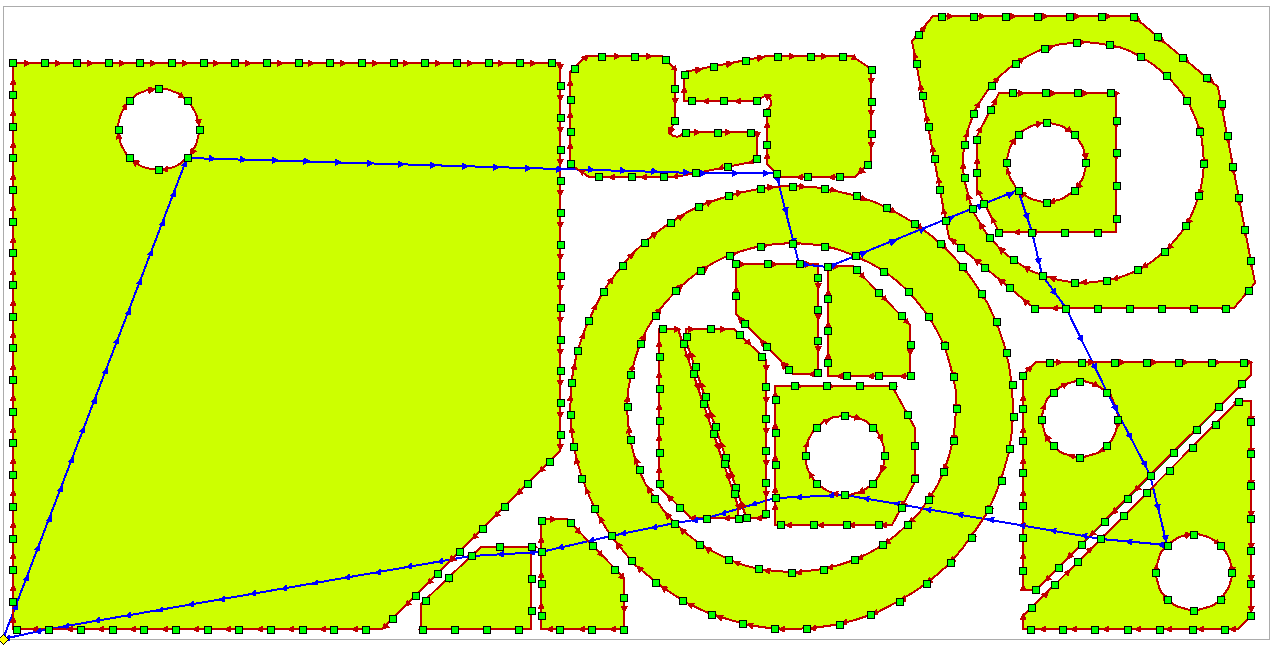
\includegraphics[width=0.95\textwidth]{464-gtsp.png}
  \end{center}
  \caption{Точное решение задачи GTSP для задания № 464}
  \label{fig:gtsp-path}
\end{figure}

\begin{figure}[p]
  \begin{center}
    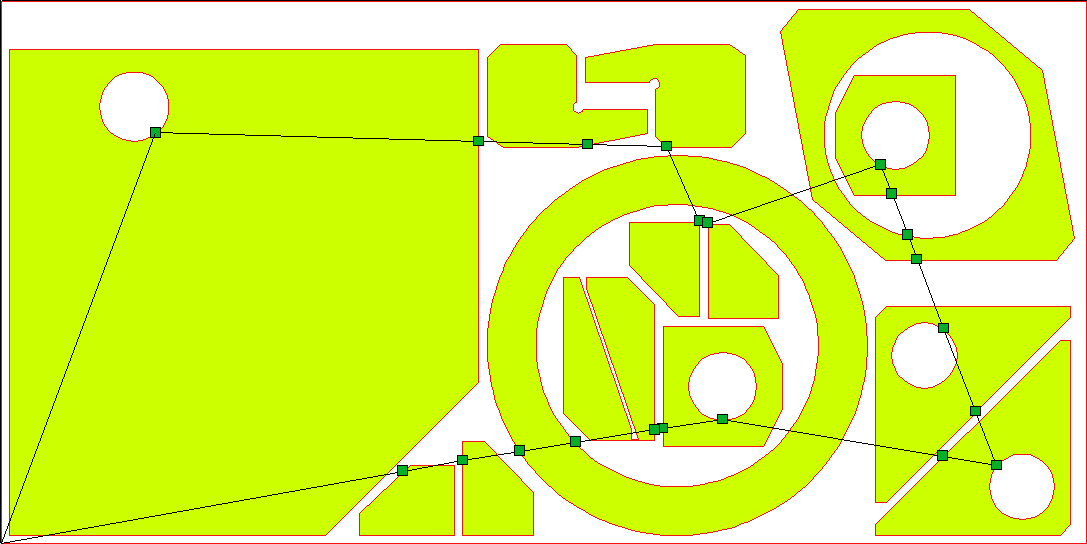
\includegraphics[width=0.95\textwidth]{464-ccp.png}
  \end{center}
  \caption{Решение задачи непрерывной резки для задания № 464}
  \label{fig:ccp-path}
\end{figure}

На рис. \ref{fig:gtsp-path}
показано точное решение задачи GTSP.
Хорошо видны возможные положения точек врезки,
которые получены путём дискретизации контура,
то есть сведения задачи непрерывной оптимизации
к задаче дискретной оптимизации.
На рис. \ref{fig:ccp-path}
показано решение задачи непрерывной резки,
полученное вышеописанным алгоритмом
для того же раскройного плана.

Видно,
что оба алгоритма дают практически идентичные
маршруты резки.
Основное отличие вызвано необходимостью дискретизации
контуров в ходе сведения задачи
непрерывной резки к GTSP.
Это приводит, в частности к тому,
что длина холостого хода в задаче GTSP
получается немного больше,
чем в задаче CCP,
что видно в табл.~\ref{tab:ccp-vs-gtsp}.
